\documentclass[11pt,]{article}
\usepackage[left=1in,top=1in,right=1in,bottom=1in]{geometry}
\newcommand*{\authorfont}{\fontfamily{phv}\selectfont}
\usepackage[]{mathpazo}


  \usepackage[T1]{fontenc}
  \usepackage[utf8]{inputenc}



\usepackage{abstract}
\renewcommand{\abstractname}{}    % clear the title
\renewcommand{\absnamepos}{empty} % originally center

\renewenvironment{abstract}
 {{%
    \setlength{\leftmargin}{0mm}
    \setlength{\rightmargin}{\leftmargin}%
  }%
  \relax}
 {\endlist}

\makeatletter
\def\@maketitle{%
  \newpage
%  \null
%  \vskip 2em%
%  \begin{center}%
  \let \footnote \thanks
    {\fontsize{18}{20}\selectfont\raggedright  \setlength{\parindent}{0pt} \@title \par}%
}
%\fi
\makeatother




\setcounter{secnumdepth}{3}

\usepackage{longtable,booktabs}

\usepackage{graphicx,grffile}
\makeatletter
\def\maxwidth{\ifdim\Gin@nat@width>\linewidth\linewidth\else\Gin@nat@width\fi}
\def\maxheight{\ifdim\Gin@nat@height>\textheight\textheight\else\Gin@nat@height\fi}
\makeatother
% Scale images if necessary, so that they will not overflow the page
% margins by default, and it is still possible to overwrite the defaults
% using explicit options in \includegraphics[width, height, ...]{}
\setkeys{Gin}{width=\maxwidth,height=\maxheight,keepaspectratio}

\title{Mis hormigas\\
Subtítulo\\
Subtítulo  }



\author{\Large Tali tali tali\vspace{0.05in} \newline\normalsize\emph{Estudiante, Universidad Autónoma de Santo Domingo (UASD)}  }


\date{}

\usepackage{titlesec}

\titleformat*{\section}{\normalsize\bfseries}
\titleformat*{\subsection}{\normalsize\itshape}
\titleformat*{\subsubsection}{\normalsize\itshape}
\titleformat*{\paragraph}{\normalsize\itshape}
\titleformat*{\subparagraph}{\normalsize\itshape}

\titlespacing{\section}
{0pt}{36pt}{0pt}
\titlespacing{\subsection}
{0pt}{36pt}{0pt}
\titlespacing{\subsubsection}
{0pt}{36pt}{0pt}





\newtheorem{hypothesis}{Hypothesis}
\usepackage{setspace}

\makeatletter
\@ifpackageloaded{hyperref}{}{%
\ifxetex
  \PassOptionsToPackage{hyphens}{url}\usepackage[setpagesize=false, % page size defined by xetex
              unicode=false, % unicode breaks when used with xetex
              xetex]{hyperref}
\else
  \PassOptionsToPackage{hyphens}{url}\usepackage[unicode=true]{hyperref}
\fi
}

\@ifpackageloaded{color}{
    \PassOptionsToPackage{usenames,dvipsnames}{color}
}{%
    \usepackage[usenames,dvipsnames]{color}
}
\makeatother
\hypersetup{breaklinks=true,
            bookmarks=true,
            pdfauthor={Tali tali tali (Estudiante, Universidad Autónoma de Santo Domingo (UASD))},
             pdfkeywords = {palabra clave 1, palabra clave 2},  
            pdftitle={Mis hormigas\\
Subtítulo\\
Subtítulo},
            colorlinks=true,
            citecolor=blue,
            urlcolor=blue,
            linkcolor=magenta,
            pdfborder={0 0 0}}
\urlstyle{same}  % don't use monospace font for urls

% set default figure placement to htbp
\makeatletter
\def\fps@figure{htbp}
\makeatother

\usepackage{pdflscape} \newcommand{\blandscape}{\begin{landscape}} \newcommand{\elandscape}{\end{landscape}}


% add tightlist ----------
\providecommand{\tightlist}{%
\setlength{\itemsep}{0pt}\setlength{\parskip}{0pt}}

\begin{document}
	
% \pagenumbering{arabic}% resets `page` counter to 1 
%
% \maketitle

{% \usefont{T1}{pnc}{m}{n}
\setlength{\parindent}{0pt}
\thispagestyle{plain}
{\fontsize{18}{20}\selectfont\raggedright 
\maketitle  % title \par  

}

{
   \vskip 13.5pt\relax \normalsize\fontsize{11}{12} 
\textbf{\authorfont Tali tali tali} \hskip 15pt \emph{\small Estudiante, Universidad Autónoma de Santo Domingo (UASD)}   

}

}








\begin{abstract}

    \hbox{\vrule height .2pt width 39.14pc}

    \vskip 8.5pt % \small 

\noindent Mi resumen


\vskip 8.5pt \noindent \emph{Keywords}: palabra clave 1, palabra clave 2 \par

    \hbox{\vrule height .2pt width 39.14pc}



\end{abstract}


\vskip 6.5pt


\noindent  \hypertarget{introducciuxf3n}{%
\section{Introducción}\label{introducciuxf3n}}

\ldots

\hypertarget{metodologuxeda}{%
\section{Metodología}\label{metodologuxeda}}

\ldots

\hypertarget{resultados}{%
\section{Resultados}\label{resultados}}

En el conjunto de la parcela, se censaron un total de 18426 individuos
pertenecientes a 16 especies. La riqueza por cuadro fue de 11 especies y
la mediana de la abundancia por cuadro fue de 328 individuos.

La especie más abundante fue \emph{Trichilia tuberculata}, con casi
11000 individuos, y las más raras fueron \emph{Pouteria fossicola} y
\emph{Rauvolfia littoralis} con 3 y 1 individuos, respectivamente. La
tabla \ref{tab:abun_sp} y la figura \ref{fig:abund_sp_q} resume estos
resultados.

\begin{longtable}[]{@{}lr@{}}
\caption{\label{tab:abun_sp}Abundancia por especie de las familia
Apocynaceae, Meliacea y Sapotaceae}\tabularnewline
\toprule
Latin & n\tabularnewline
\midrule
\endfirsthead
\toprule
Latin & n\tabularnewline
\midrule
\endhead
Trichilia tuberculata & 10842\tabularnewline
Guarea guidonia & 1889\tabularnewline
Tabernaemontana arborea & 1732\tabularnewline
Pouteria reticulata & 1084\tabularnewline
Guarea bullata & 725\tabularnewline
Chrysophyllum argenteum & 711\tabularnewline
Aspidosperma spruceanum & 473\tabularnewline
Trichilia pallida & 472\tabularnewline
Chrysophyllum cainito & 171\tabularnewline
Lacmellea panamensis & 102\tabularnewline
Thevetia ahouai & 84\tabularnewline
Guarea grandifolia & 65\tabularnewline
Pouteria stipitata & 60\tabularnewline
Cedrela odorata & 12\tabularnewline
Pouteria fossicola & 3\tabularnewline
Rauvolfia littoralis & 1\tabularnewline
\bottomrule
\end{longtable}

\begin{figure}
\centering
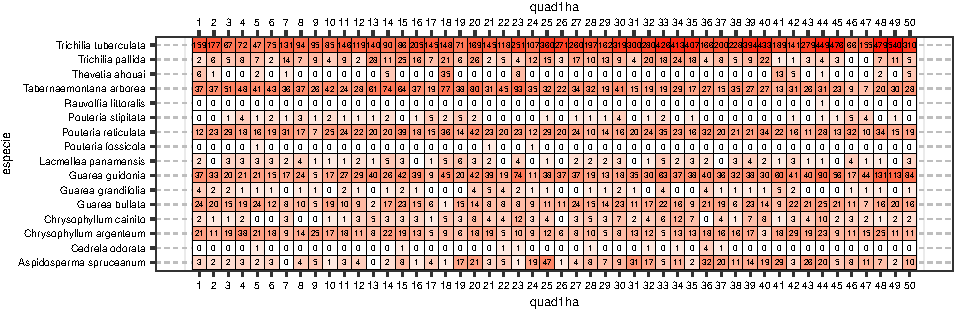
\includegraphics{manuscrito_files/figure-latex/unnamed-chunk-3-1.pdf}
\caption{\label{fig:abun_sp_q}Abundancia por especie por quadrat}
\end{figure}

\hypertarget{discusiuxf3n}{%
\section{Discusión}\label{discusiuxf3n}}

\hypertarget{agradecimientos}{%
\section{Agradecimientos}\label{agradecimientos}}

\hypertarget{informaciuxf3n-de-soporte}{%
\section{Información de soporte}\label{informaciuxf3n-de-soporte}}

\ldots

\hypertarget{script-reproducible}{%
\section{\texorpdfstring{\emph{Script}
reproducible}{Script reproducible}}\label{script-reproducible}}

\ldots

\hypertarget{referencias}{%
\section{Referencias}\label{referencias}}




\newpage
\singlespacing 
\end{document}
